\clearpage 

\section {Construction of Feldman-Cousins confidence regions}
\label{sec:fc}

The best-fit $|\Delta m^{2}_{23}|$ fluctuation seen in the analysis of the Run1 dataset is no longer present
(see Figs.\ \ref{fig:genie_deltachisq_dmsq_wide_3datasets} and \ref{fig:neut_deltachisq_dmsq_wide_3datasets}).
The analysis of the Run2 and the combined Run1+2 datasets strongly disfavours any interpretation of the 
observed 1 $\mu$-like ring event deficit in terms of large $|\Delta m^{2}_{23}|$ (a second or higher-order oscillation maximum 
at $\sim$600 MeV). Therefore, for reasons of {\em computational efficiency}, we limit the Feldman-Cousins
construction to the $|\Delta m^{2}_{23}|$ range from 1$\times$10$^{-3}$ $eV^{2}/c^{4}$ to 6$\times$10$^{-3}$ $eV^{2}/c^{4}$.

The application of the Feldman-Cousins method \cite{FeldmanCousins} to the T2K $\nu_{\mu}$-disappearance analysis
is discussed in detail in Sec. 3.4 of Ref. \cite{OurRun1DisappAnalysis}:
a number of toy MC experiment fits is performed for each point of the (sin$^{2}$2$\theta_{23}$, $|\Delta$m$^{2}_{23}|$)
2-dimensional grid.
For each grid point, the critical value of $\Delta\chi^{2}$ ($\Delta\chi^{2}_{critical}$)
is found such that $\alpha$ of the toy MC experiments have $\Delta\chi^{2}_{MC}$ $<$ $\Delta\chi^{2}_{critical}$,
where $\alpha$ is the desired confidence level (see Fig. \ref{fig:minos2011_dchisq_cumulative}).
The value of $\Delta\chi^{2}_{MC}$ for each toy MC experiment is calculated as follows:
\begin{equation}
\displaystyle
\Delta \chi^{2}_{MC} = \chi^{2} \textrm{(true)} - \chi^{2} \textrm{(MC, best-fit)}
\label{eq:deltachi2}
\end{equation}
where
``true'' means the true values of the oscillation parameters at that grid point, and
``best-fit'' means the best-fit values for that MC experiment (this is equivalent to 
equation 5.6 in \cite{FeldmanCousins}).
$\chi^{2}$ is defined as
\begin{equation}
\displaystyle
\chi^{2} (sin^{2}2\theta_{23},|\Delta m^{2}_{23}|;{\bf a}) =
  2 \cdot \sum_{i=0}^{N-1}
   \Big(
     n^{obs}_{i} \cdot ln(n^{obs}_{i}/n^{exp}_{i}) +
     (n^{exp}_{i}-n^{obs}_{i})
   \Big) 
\label{eq:chisquare}
\end{equation}
where
$N$ is the number of reconstructed energy bins,
${\bf a}$ is a vector of nuisance parameters (see Tab. \ref{tab:input_uncertainties}),
$n^{obs}_{i}$ is the observed number of events in the $i^{th}$ bin, and
$n^{exp}_{i} = n^{exp}_{i}(sin^{2}2\theta_{23},\Delta m^{2}_{23}; {\bf a})$
is the corresponding expected number of events. This definition of $\chi^{2}$ arises from our use
of the likelihood ratio method, which is explained in more detail in 
Sec.\ 3.2 of Ref.\ \cite{OurRun1DisappAnalysis}.

\section {Run 1+2 oscillation parameter confidence regions }
\label{sec:conf_regions}

Feldman-Cousins confidence regions were constructed using the 
$\Delta\chi^{2}$(sin$^{2}$2$\theta_{23}$, $|\Delta$m$^{2}_{23}|$) surfaces
from the fits presented in Sec.\ \ref{sec:fits} and the
$\Delta\chi^{2}_{critical}$(sin$^{2}$2$\theta_{23}$, $|\Delta$m$^{2}_{23}|$) maps
presented in Sec.\ \ref{sec:fc}.

The 68\% and 90\% Feldman-Cousins confidence regions are shown for the
2-flavour $\nu_{\mu}$-disappearance fit to the combined Run1+2 dataset 
with and without systematics
in Fig.\ \ref{fig:contour_run1p2_statsyst_genie} for GENIE and
in Fig.\ \ref{fig:contour_run1p2_statsyst_neut} for NEUT.
(It is worth noting that all confidence regions presented here are drawn
using a $sin^{2}2\theta_{23}$ bin size of 0.01 and 
a $|\Delta m^{2}_{23}|$ bin size of 1.0$\times10^{-4}$ $eV^{2}/c^{4}$).
The star-shaped marker in each plot marks the bin with the minimum $\chi^{2}$.)
The 90\% confidence regions are compared with those from 
MINOS \cite{Minos2011} and SuperK \cite{OldDisappSuperK}
in Fig.\ \ref{fig:contour_run1p2_statsyst_genie_external_90cl} for GENIE and
in Fig.\ \ref{fig:contour_run1p2_statsyst_neut_external_90cl} for NEUT.
A similar comparison is shown in Figs.
\ref{fig:contour_run1p2_statsyst_genie_external} and
\ref{fig:contour_run1p2_statsyst_neut_external}, and
includes the 68\% confidence regions from T2K and MINOS.

In Fig.\ \ref{fig:contour_run1p2_statsyst_genie_minos11sens}
the 90\% Feldman-Cousins confidence region (with systematics) from the GENIE
2-flavour $\nu_{\mu}$-disappearance fit to the combined Run1+2 dataset 
is compared with the T2K $1.431 \times 10^{20}$ POT sensitivity for oscillations
with the 2011 MINOS best-fit values
($sin^{2}2\theta_{23}$ = 1.0 and $|\Delta m^{2}_{23}|$ = 2.32$\times10^{-3}$ $eV^{2}/c^{4}$).
The 2011 MINOS 90\% confidence region is also shown in this figure.
The equivalent comparison from the NEUT 2-flavour $\nu_{\mu}$-disappearance fit is shown in 
Fig.\ \ref{fig:contour_run1p2_statsyst_neut_minos11sens}.

The 90\% Feldman-Cousins confidence region from the fit to the combined Run1+2 dataset
is compared with the 90\% confidence regions from the fits to the Run1-only and Run2-only datasets 
in Fig.\ \ref{fig:contour_statsyst_genie_3datasets} for GENIE and
in Fig.\ \ref{fig:contour_statsyst_neut_3datasets} for NEUT.

Finally, a comparison of the GENIE and NEUT 90\% Feldman-Cousins confidence regions 
from the fit to the combined Run1+2 dataset 
is shown in Fig.\ \ref{fig:contour_statsyst_genie_neut_comparison}.


%
% --------------------------------------------------------------------------------------------------------------------
%

% plot moved to previous section (numuosc2_contours.tex) to avoid having 2 half-empty pages
%
%\begin{figure*}[htb]
%\center
%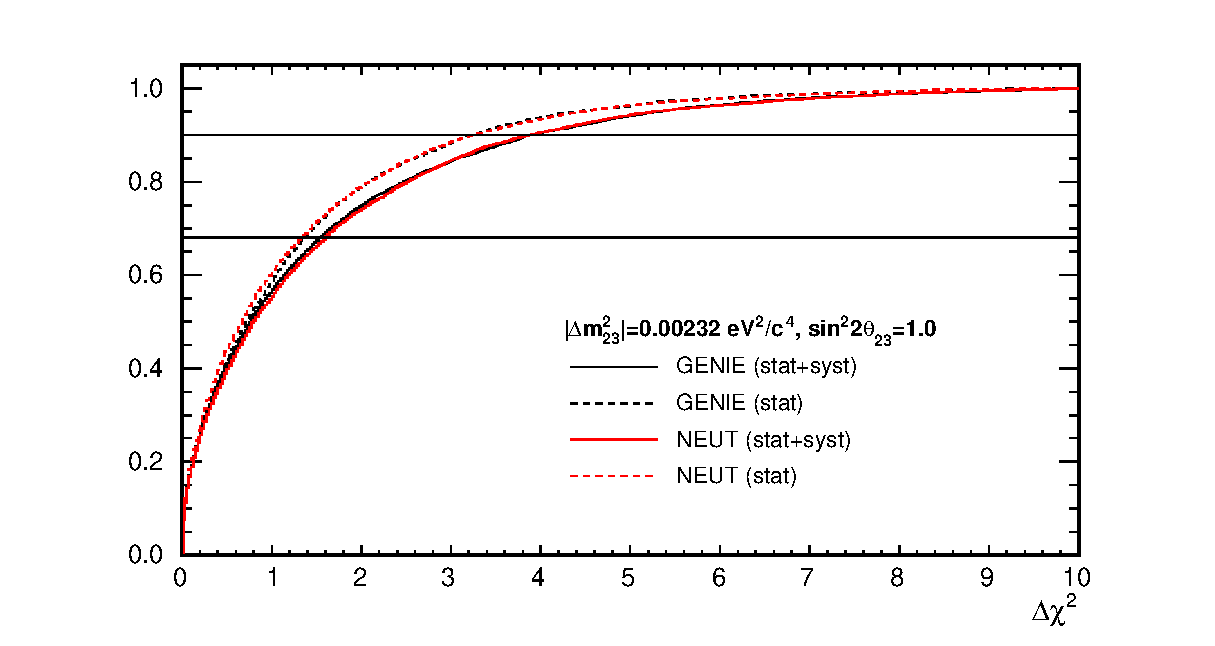
\includegraphics[width=24pc]{./images/feldman_cousins/minos2011_dchisq_cummulative.eps}
%\caption{
%  Cumulative $\Delta\chi^{2}_{MC}$ distributions (for both NEUT and GENIE) for oscillated toy MC experiments generated
%  with $sin^{2}2\theta_{23}$ = 1.0 and $|\Delta m^{2}_{23}|$ = 2.32$\times10^{-3}$ $eV^{2}/c^{4}$.
%  The horizontal lines show the 68\% and 90\% levels
%  (values of $\Delta\chi^{2}_{critical}$ are the values of $\Delta\chi^{2}_{MC}$ where these horizontal lines
%  intersect with the cumulative distributions).
%}
%\label{fig:minos2011_dchisq_cumulative}
%\end{figure*}

\begin{figure*}[htb]
\center
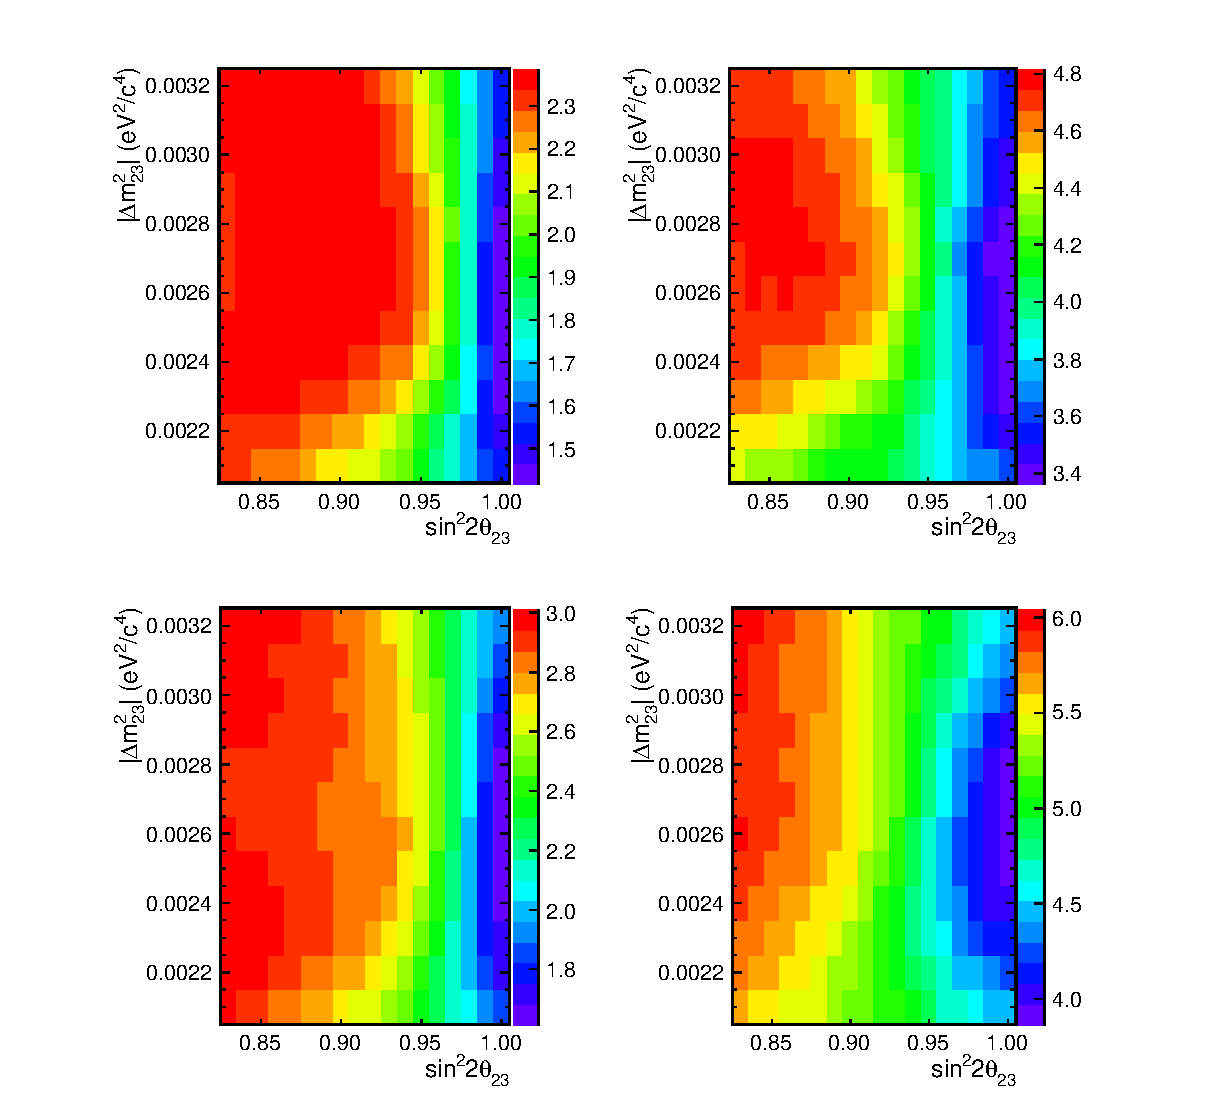
\includegraphics[width=42pc]{./images/feldman_cousins/fc_deltachisqcrit_2d_neut.eps}
\caption{
  Monte Carlo estimation,
  according to the Feldman-Cousins method,
  of $\Delta\chi^{2}_{68}$ (left) and $\Delta\chi^{2}_{90}$ (right)
  as functions of $sin^{2}{2\theta_{23}}$ and $\Delta{m^{2}_{23}}$,
  for calculation of the 68\% (left) and 90\% (right) CL confidence regions
  for the $1.431 \times 10^{20}$-POT T2K 2-flavour $\nu_{\mu}$-disappearance analysis.
  The top row shows $\Delta\chi^{2}$ surfaces calculated using statistical fluctuations
  only whereas the bottom row shows $\Delta\chi^{2}$ surfaces calculated using
  both systematic variations and statistical fluctations.
  As expected from \cite{FeldmanCousins}, the values of $\Delta\chi^{2}$ 
  decrease as the
  physical boundary at $sin^{2}{2\theta_{23}}$ = 1 is approached. 
}
\label{fig:fc_deltachisqcrit_2d_neut}
\end{figure*}


\begin{figure*}[htb]
\center
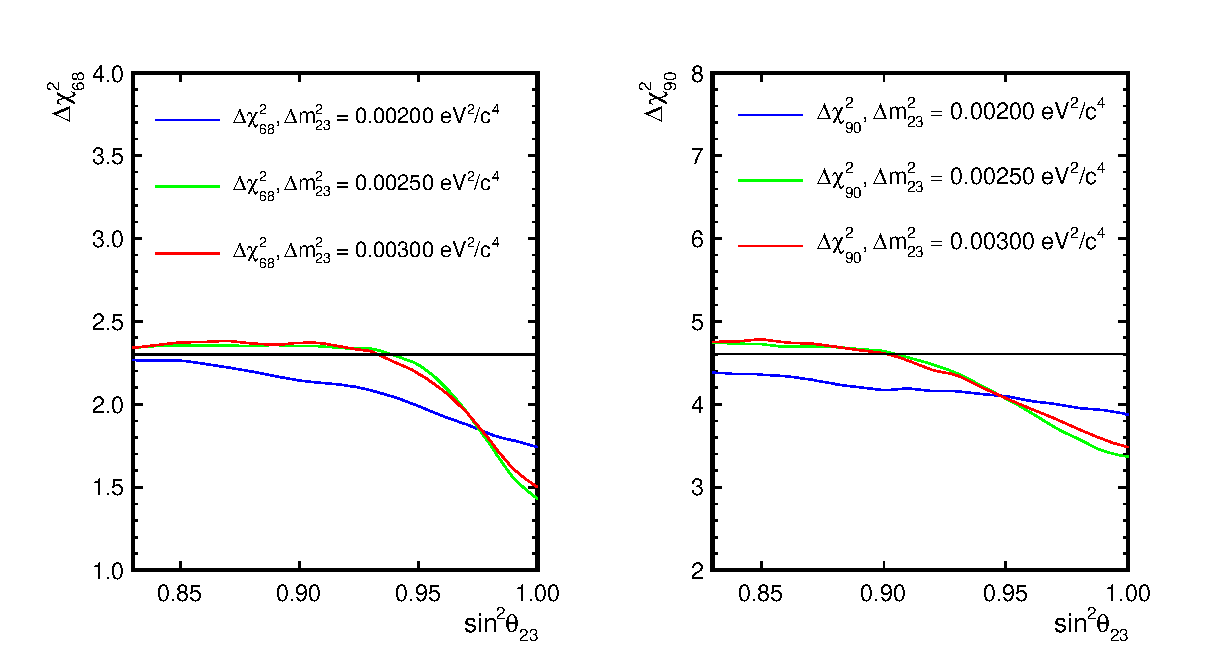
\includegraphics[width=38pc]{./images/feldman_cousins/fc_deltachisqcrit_statonly_vs_sinsq_3dmsq_neut.eps}
\caption{
  Monte Carlo estimation,
  according to the Feldman-Cousins method (statistical errors only),
  of $\Delta\chi^{2}_{68}$ (left) and $\Delta\chi^{2}_{90}$ (right),
  as functions of $sin^{2}{2\theta_{23}}$ for 3 different values of $\Delta{m^{2}_{23}}$
  ($2.0 \times 10^{-3} eV^{2}/c^{4}$,
   $2.5 \times 10^{-3} eV^{2}/c^{4}$ and
   $3.0 \times 10^{-3} eV^{2}/c^{4}$).
  For comparison, the canonical value of $\Delta\chi^{2}$ used in the constant $\Delta\chi^{2}_{critical}$
  method is also shown as a horizontal line.
}
\label{fig:fc_deltachisqcrit_statonly_vs_sinsq_3dmsq_neut}
\end{figure*}

\begin{figure*}[htb]
\center
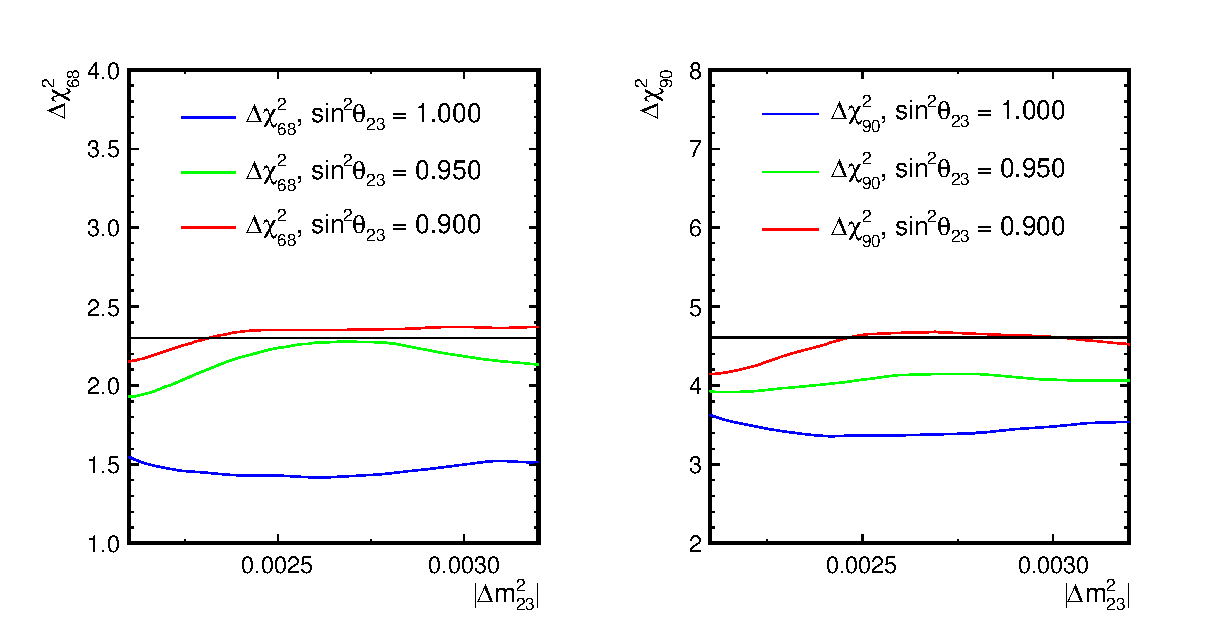
\includegraphics[width=38pc]{./images/feldman_cousins/fc_deltachisqcrit_statonly_vs_dmsq_3sinsq_neut.eps}
\caption{
  Monte Carlo estimation,
  according to the Feldman-Cousins method (statistical errors only),
  of $\Delta\chi^{2}_{68}$ (left) and $\Delta\chi^{2}_{90}$ (right),
  as functions of $\Delta{m^{2}_{23}}$ for 3 different values of $sin^{2}{2\theta_{23}}$
  (0.90, 0.95 and 1.00).
  For comparison, the canonical value of $\Delta\chi^{2}$ used in the constant $\Delta\chi^{2}_{critical}$
  method is also shown as a horizontal line.
}
\label{fig:fc_deltachisqcrit_statonly_vs_dmsq_3sinsq_neut}
\end{figure*}



%
% confidence regions for the Run1+2 fit
%

\begin{figure*}[htb]
\center
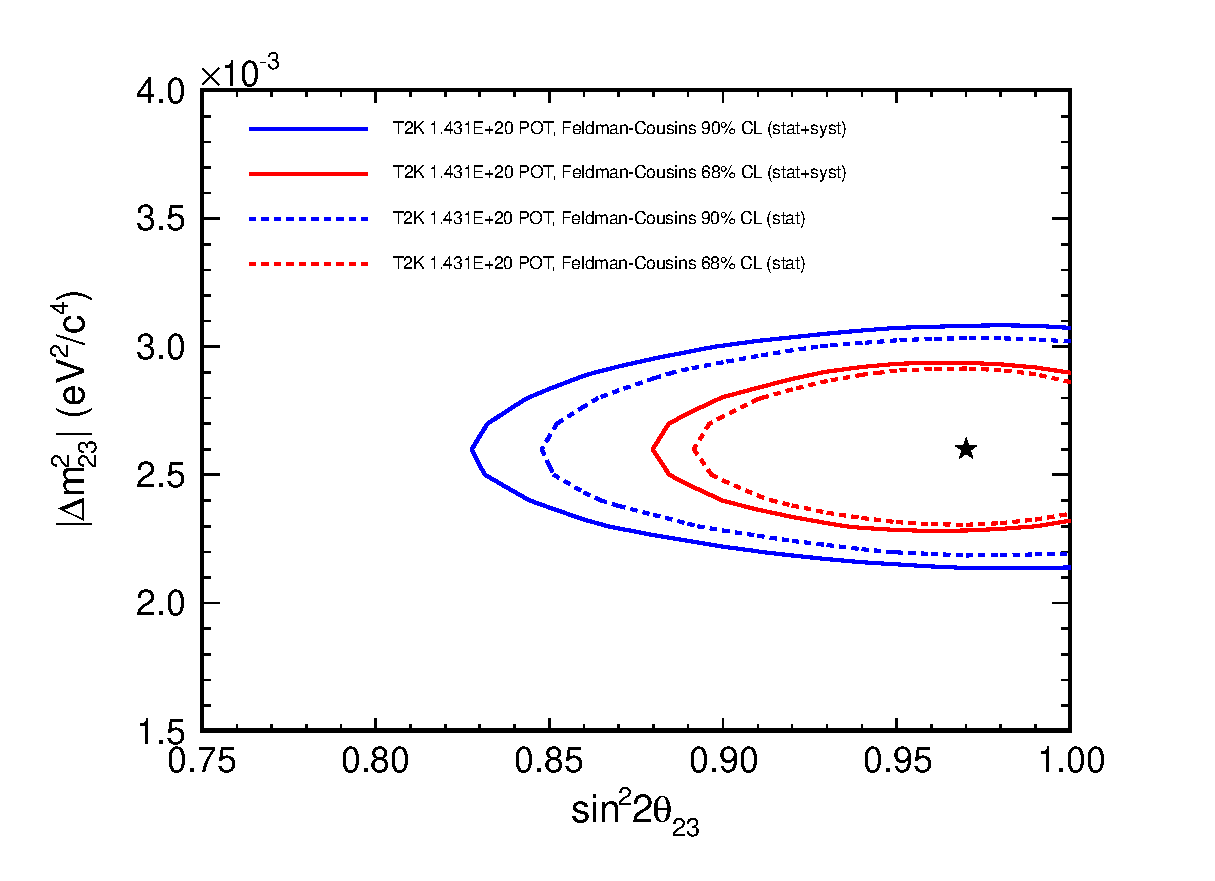
\includegraphics[width=30pc]{./images/confidence_regions/contour_run1p2_statsyst_genie.eps}
\caption{
  68\% and 90\% Feldman-Cousins confidence regions, with and without systematics,
  for the GENIE 2-flavour $\nu_{\mu}$-disappearance fit to the combined Run1+2 dataset
}
\label{fig:contour_run1p2_statsyst_genie}
\end{figure*}


\begin{figure*}[htb]
\center
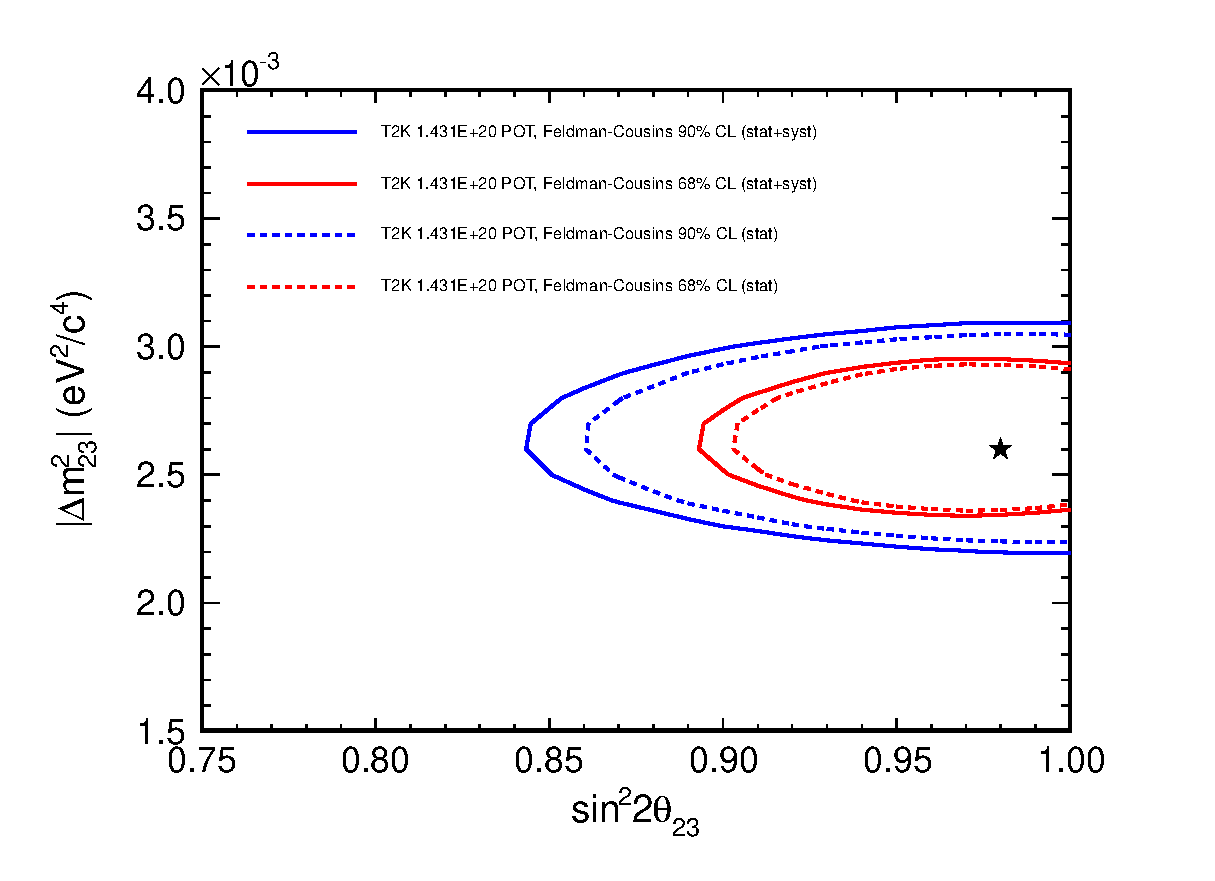
\includegraphics[width=30pc]{./images/confidence_regions/contour_run1p2_statsyst_neut.eps}
\caption{
  68\% and 90\% Feldman-Cousins confidence regions, with and without systematics,
  for the NEUT 2-flavour $\nu_{\mu}$-disappearance fit to the combined Run1+2 dataset
}
\label{fig:contour_run1p2_statsyst_neut}
\end{figure*}

%
% confidence regions for the Run1+2 fit - comparison with MINOS/K2K/SK-atm
%

\begin{figure*}[htb]
\center
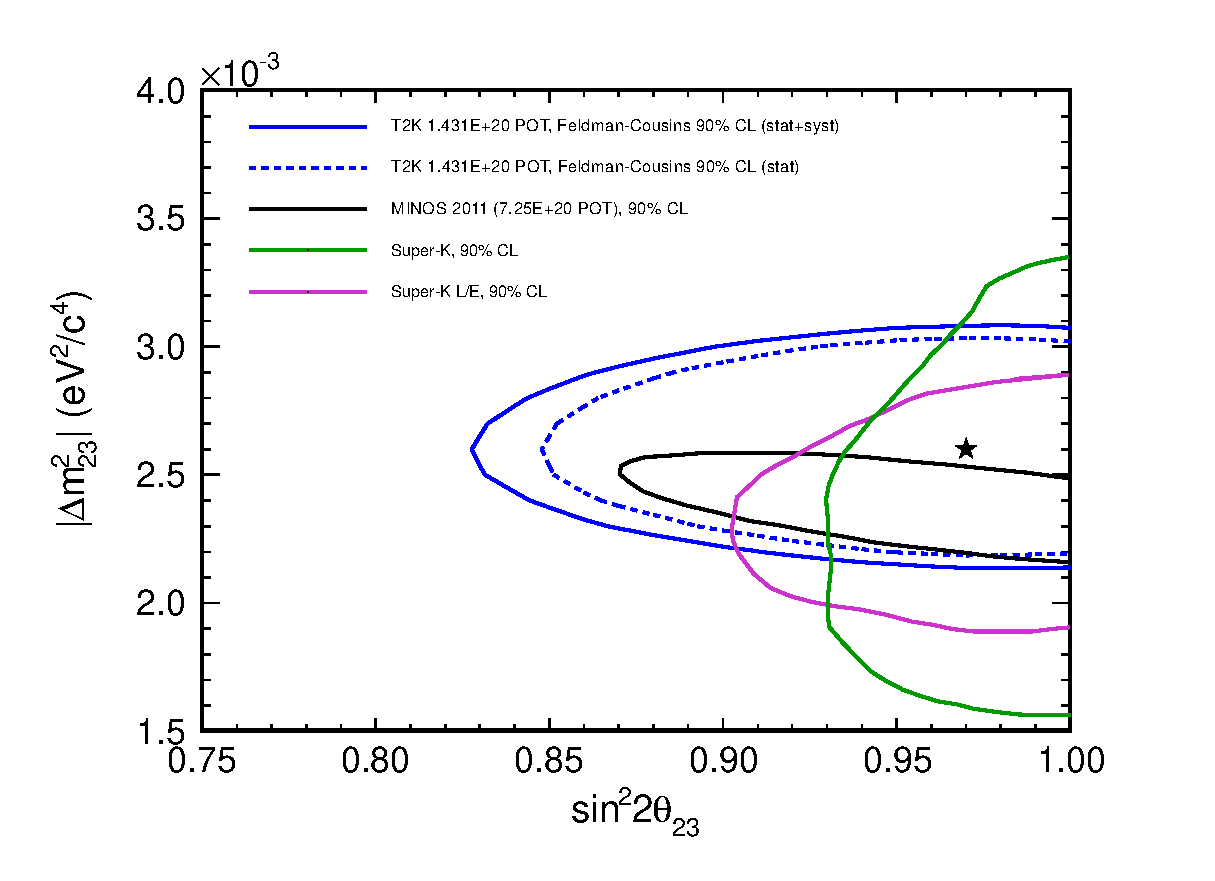
\includegraphics[width=30pc]{./images/confidence_regions/contour_run1p2_statsyst_genie_external_90clonly.eps}
\caption{
  90\% Feldman-Cousins confidence regions, with and without systematics,
  for the GENIE 2-flavour $\nu_{\mu}$-disappearance fit to the combined Run1+2 dataset:
  comparisons with results from MINOS \cite{Minos2011} and SuperK \cite{OldDisappSuperK}.
}
\label{fig:contour_run1p2_statsyst_genie_external_90cl}
\end{figure*}

\begin{figure*}[htb]
\center
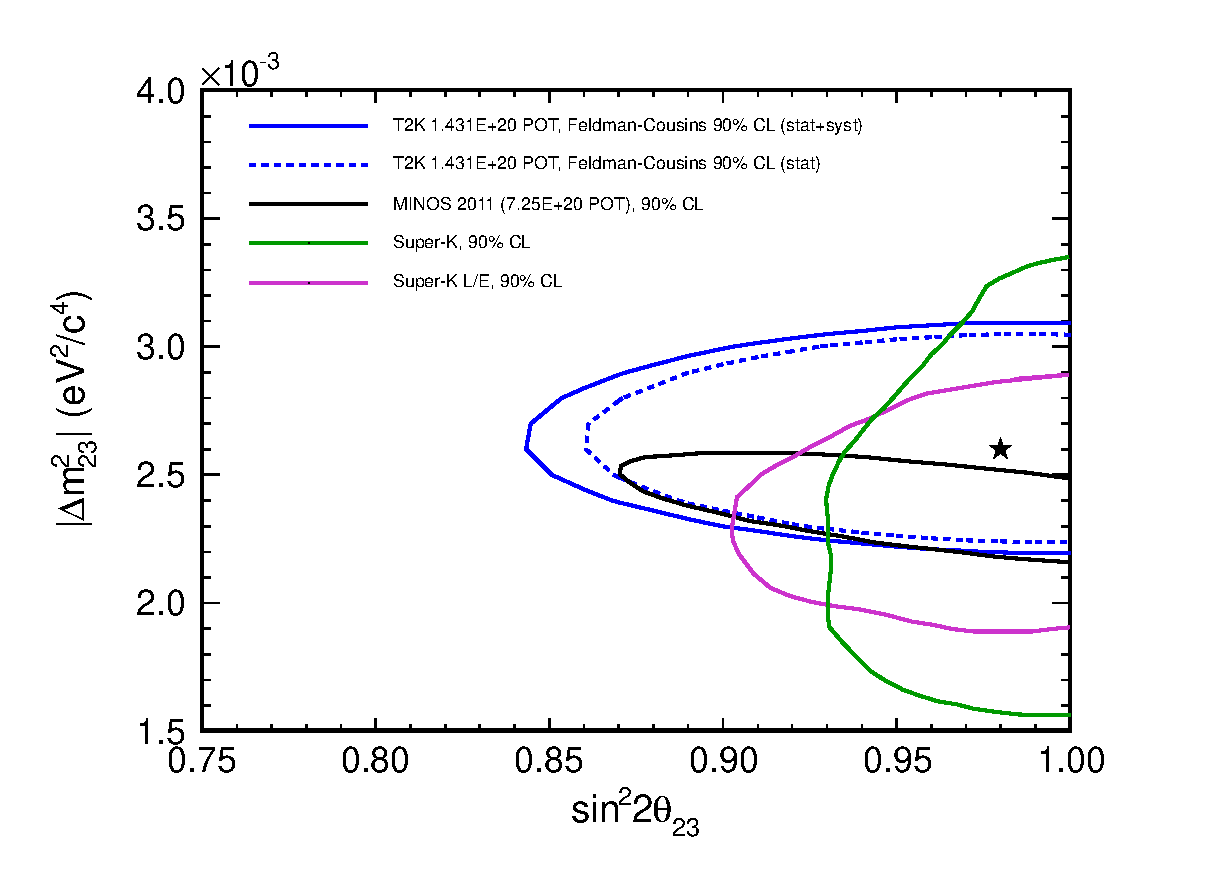
\includegraphics[width=30pc]{./images/confidence_regions/contour_run1p2_statsyst_neut_external_90clonly.eps}
\caption{
  90\% Feldman-Cousins confidence regions, with and without systematics,
  for the NEUT 2-flavour $\nu_{\mu}$-disappearance fit to the combined Run1+2 dataset:
  comparisons with results from MINOS \cite{Minos2011} and SuperK \cite{OldDisappSuperK}.
}
\label{fig:contour_run1p2_statsyst_neut_external_90cl}
\end{figure*}


%
% confidence regions for the Run1+2 fit - comparison with MINOS/K2K/SK-atm
%

\begin{figure*}[htb]
\center
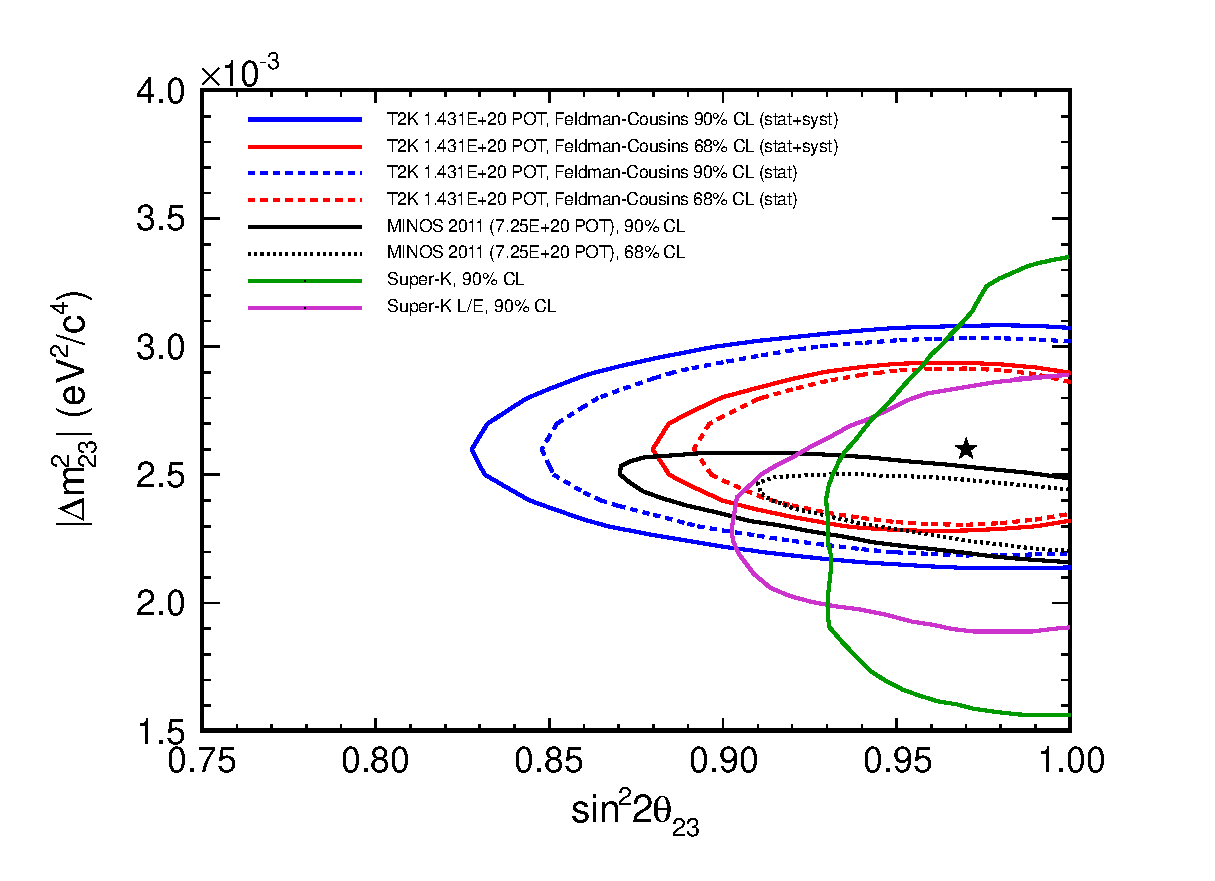
\includegraphics[width=30pc]{./images/confidence_regions/contour_run1p2_statsyst_genie_external.eps}
\caption{
  68\% and 90\% Feldman-Cousins confidence regions, with and without systematics,
  for the GENIE 2-flavour $\nu_{\mu}$-disappearance fit to the combined Run1+2 dataset:
  comparisons with MINOS 2011 68\% and 90\% contours \cite{Minos2011} and SuperK 90\% contour \cite{OldDisappSuperK}.
}
\label{fig:contour_run1p2_statsyst_genie_external}
\end{figure*}

\begin{figure*}[htb]
\center
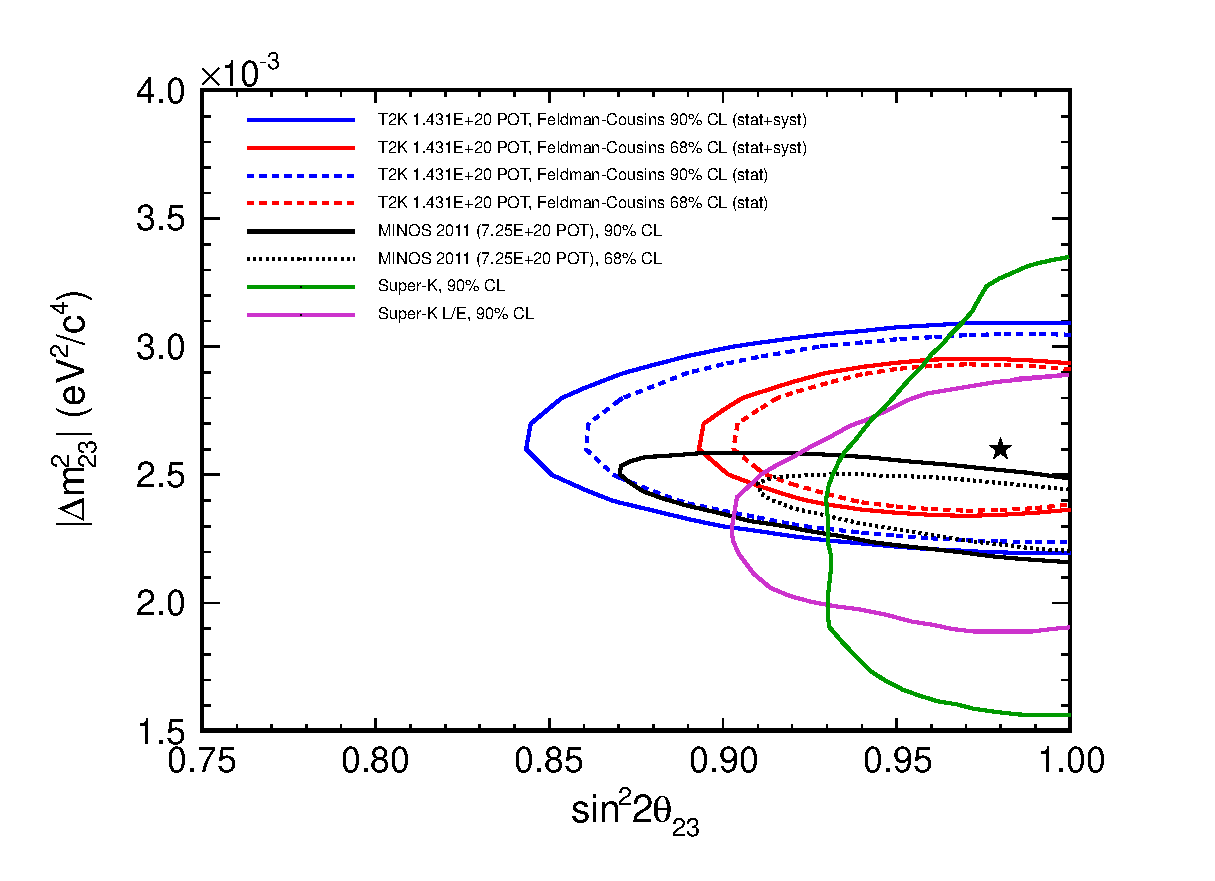
\includegraphics[width=30pc]{./images/confidence_regions/contour_run1p2_statsyst_neut_external.eps}
\caption{
  68\% and 90\% Feldman-Cousins confidence regions, with and without systematics,
  for the NEUT 2-flavour $\nu_{\mu}$-disappearance fit to the combined Run1+2 dataset:
  comparisons with MINOS 2011 68\% and 90\% contours \cite{Minos2011} and SuperK 90\% contour \cite{OldDisappSuperK}.
}
\label{fig:contour_run1p2_statsyst_neut_external}
\end{figure*}


%
% confidence regions for the Run1+2 fit - comparison with sensitivity for MINOS-2011 params
%

\begin{figure*}[htb]
\center
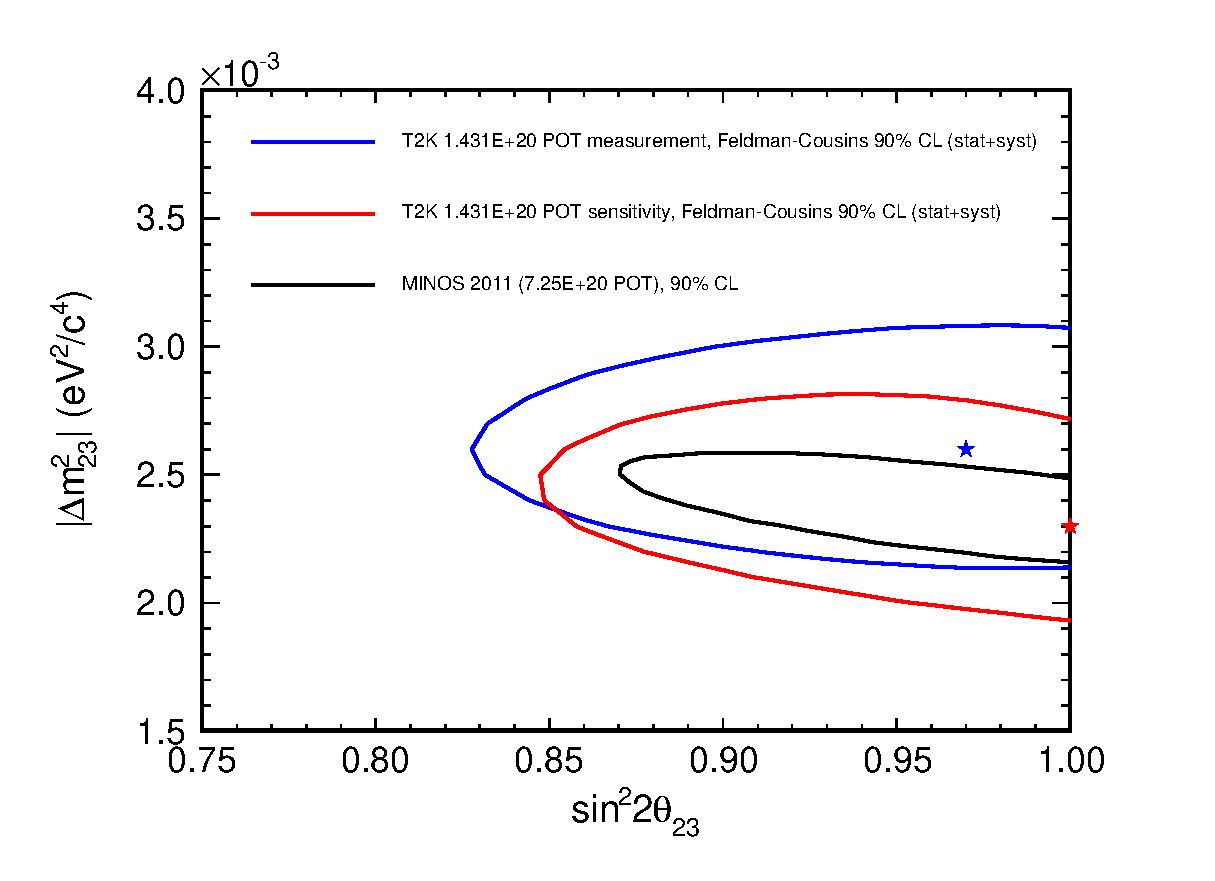
\includegraphics[width=30pc]{./images/confidence_regions/contour_run1p2_statsyst_genie_minos11sens.eps}
\caption{
  90\% Feldman-Cousins confidence regions (with systematics)
  for the GENIE 2-flavour $\nu_{\mu}$-disappearance fit to the combined Run1+2 dataset:
  comparisons with T2K 1.431$\times$10$^{20}$ POT sensitivity for $\nu_{\mu}$-disappearance with the MINOS 2011 
  best-fit values ($sin^{2}2\theta_{23}$ = 1.0 and $|\Delta m^{2}_{23}|$ = 2.32$\times10^{-3}$ $eV^{2}/c^{4}$).
  The MINOS 2011 90\% confidence region \cite{Minos2011} is also shown.
}
\label{fig:contour_run1p2_statsyst_genie_minos11sens}
\end{figure*}

\begin{figure*}[htb]
\center
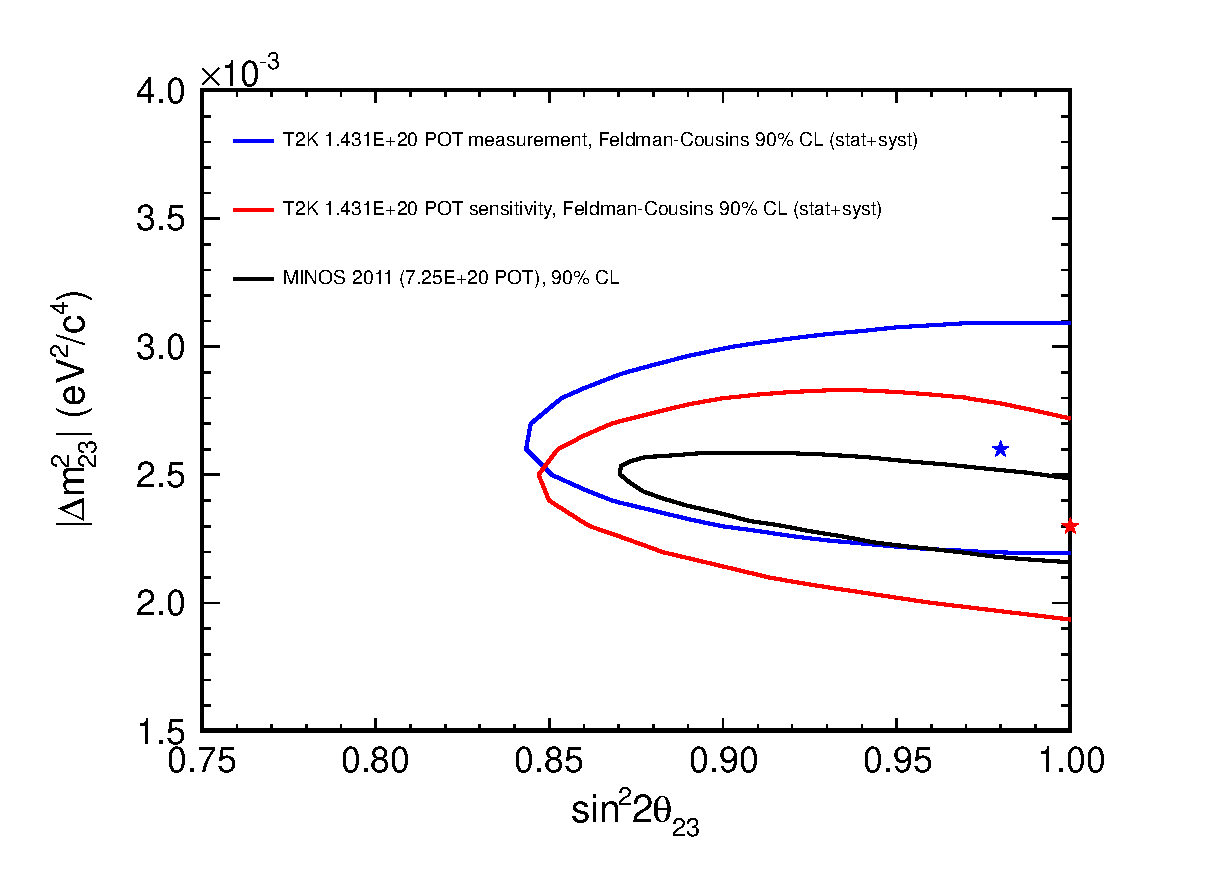
\includegraphics[width=30pc]{./images/confidence_regions/contour_run1p2_statsyst_neut_minos11sens.eps}
\caption{
  90\% Feldman-Cousins confidence regions (with systematics)
  for the NEUT 2-flavour $\nu_{\mu}$-disappearance fit to the combined Run1+2 dataset:
  comparisons with T2K 1.431$\times$10$^{20}$ POT sensitivity for $\nu_{\mu}$-disappearance with the MINOS 2011 
  best-fit values ($sin^{2}2\theta_{23}$ = 1.0 and $|\Delta m^{2}_{23}|$ = 2.32$\times10^{-3}$ $eV^{2}/c^{4}$).
  The MINOS 2011 90\% confidence region \cite{Minos2011} is also shown.
}
\label{fig:contour_run1p2_statsyst_neut_minos11sens}
\end{figure*}



%
% confidence regions for the Run1, Run2 and Run1+2 fits
%

\begin{figure*}[htb]
\center
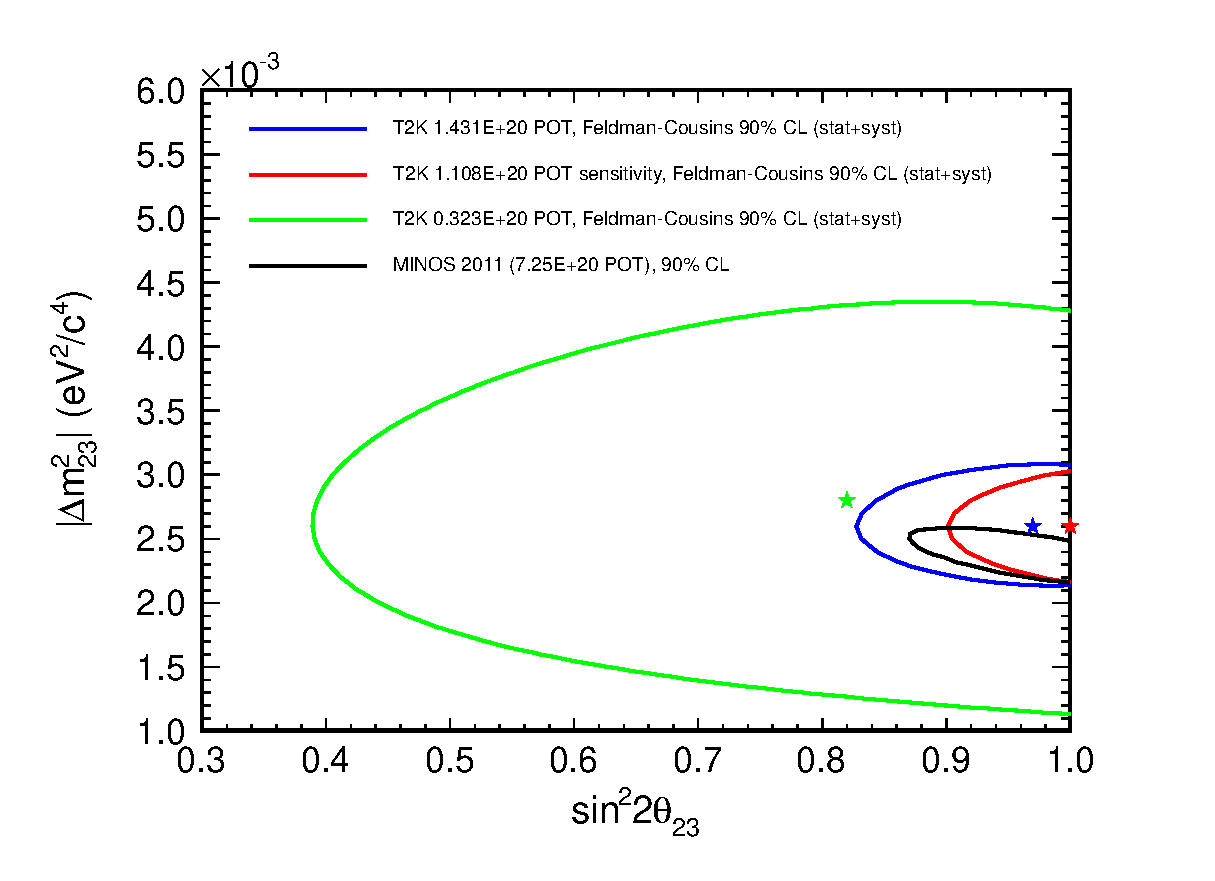
\includegraphics[width=30pc]{./images/confidence_regions/contour_statsyst_genie_3datasets.eps}
\caption{
  90\% Feldman-Cousins confidence regions (with systematics)
  for the GENIE 2-flavour $\nu_{\mu}$-disappearance fits to the Run1, Run2 and the combined Run1+2 datasets.
  The MINOS 2011 result \cite{Minos2011} is also shown for reference.
}
\label{fig:contour_statsyst_genie_3datasets}
\end{figure*}

\begin{figure*}[htb]
\center
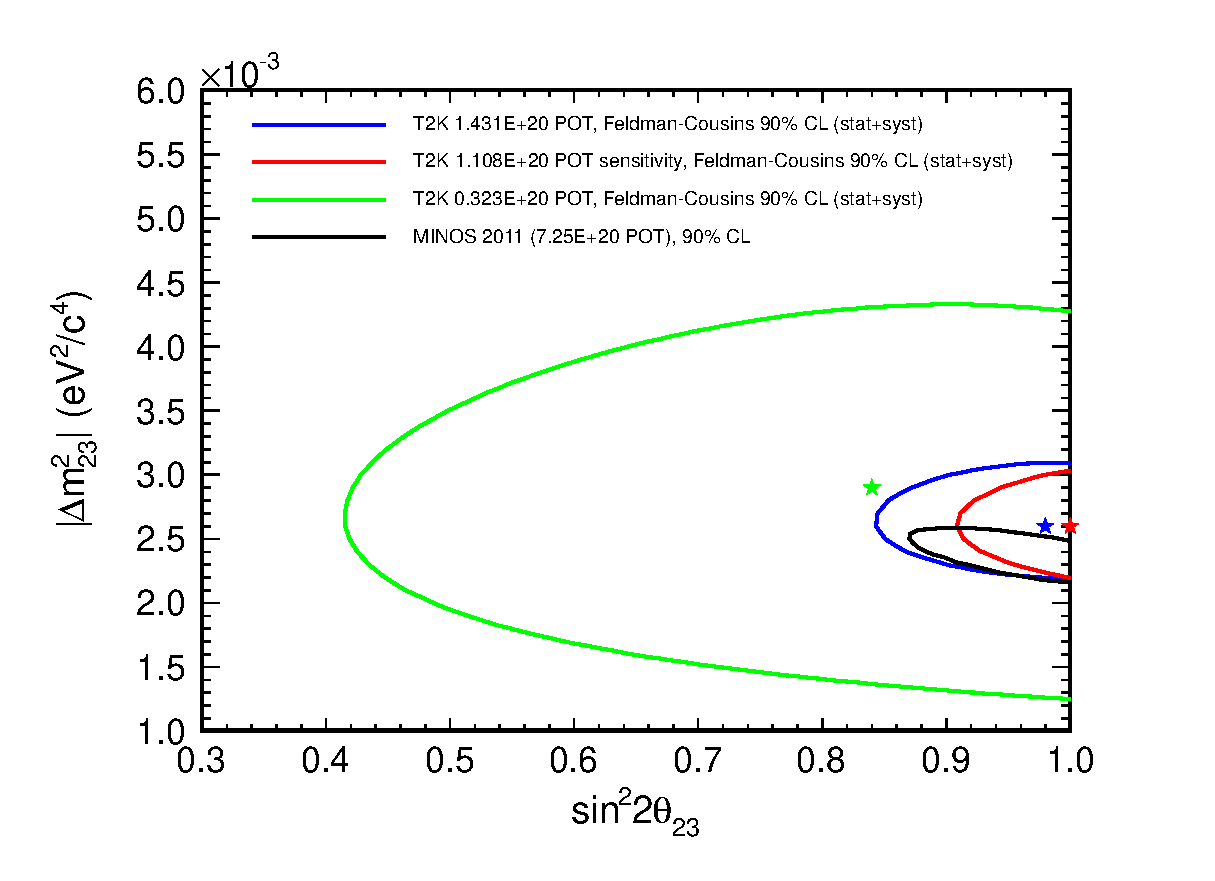
\includegraphics[width=30pc]{./images/confidence_regions/contour_statsyst_neut_3datasets.eps}
\caption{
  90\% Feldman-Cousins confidence regions (with systematics)
  for the NEUT 2-flavour $\nu_{\mu}$-disappearance fits to the Run1, Run2 and the combined Run1+2 datasets.
  The MINOS 2011 result \cite{Minos2011} is also shown for reference.
}
\label{fig:contour_statsyst_neut_3datasets}
\end{figure*}


%
% comparison of GENIE and NEUT Run1+2 contours
%

\begin{figure*}[htb]
\center
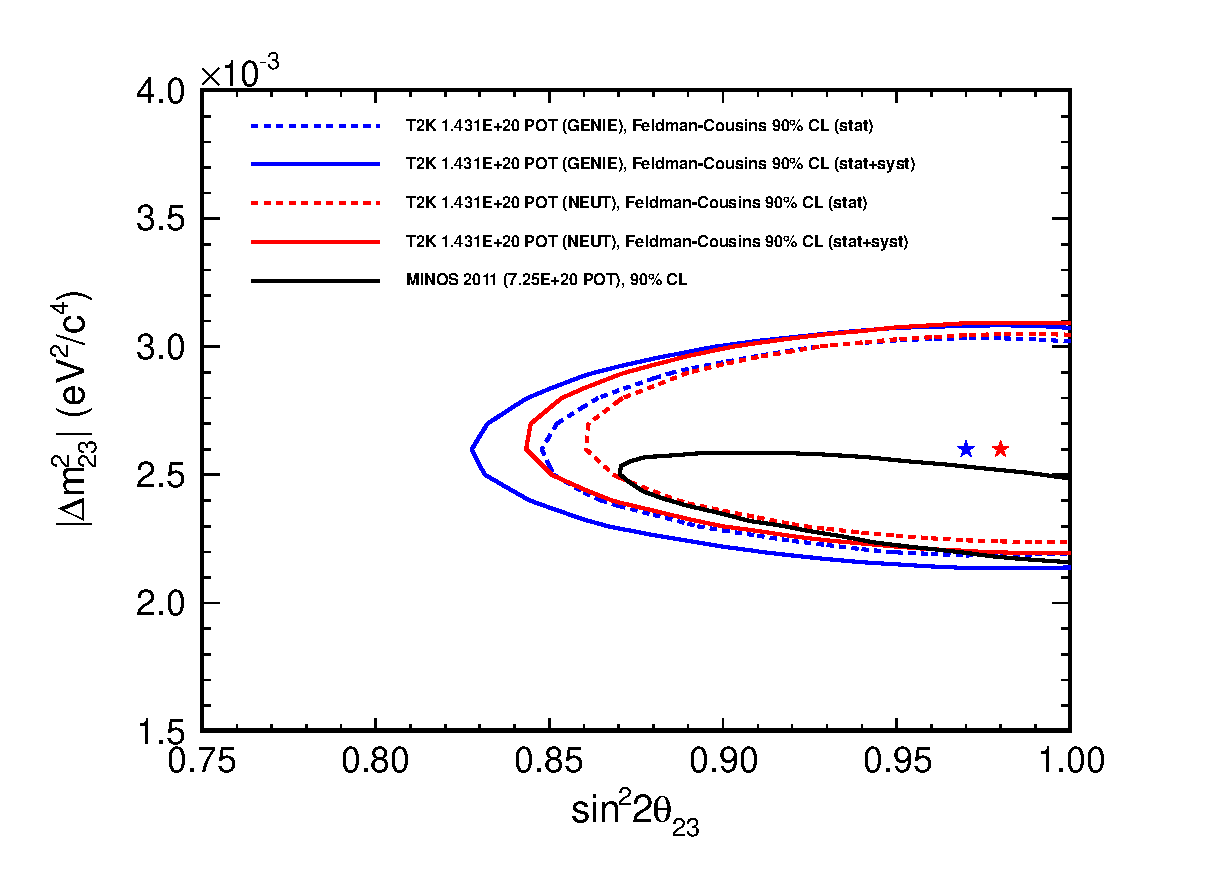
\includegraphics[width=30pc]{./images/confidence_regions/contour_run1p2_genie_neut_comparison.eps}
\caption{
  Comparison of the GENIE and NEUT 90\% Feldman-Cousins confidence regions (with and witout systematics)
  for the 2-flavour $\nu_{\mu}$-disappearance fits to the combined Run1+2 dataset.
  The MINOS 2011 result \cite{Minos2011} is also shown for reference.
}
\label{fig:contour_statsyst_genie_neut_comparison}
\end{figure*}

